\documentclass{MScthesisITEM}

% this package is just to generate text for demo-purposes
\usepackage{blindtext}
\usepackage{hyperref}
\usepackage{glossaries}
\usepackage{graphicx}


\title{iPhone Application 
\newlinetitle for Controlling Wireless Access Point} % The title of your assignement; NB use \newlinetitle to start a newline
\author{Xiao Chen} % Your firstname and lastname
\professor{Bjrn J. Villa, ITEM} % Affiliation = ITEM for instance
\supervisor{Poul E Heegaard, ITEM}

%% Uncomment the following in case you want subfigures; note that there will be a warning for the caption package
% \let\subcaption\undefined
% \let\subfloat\undefined
% \usepackage[bf]{caption}
% \usepackage{subcaption}

\DeclareGraphicsExtensions{.pdf,.jpg,.png}
\graphicspath{{./figs/}}

%% \loadglsentries{glossary}
\pagestyle{empty}

\newacronym{ntnu}{NTNU}{Norwegian University of Science and Technology}

\newacronym{rpi}{RPI}{Raspberry Pi}

\newacronym{ios}{IOS}{iPhone Operation System}

\newacronym{sd}{SD}{Secure Digital}

\newacronym{item}{ITEM}{Telematics}

\newacronym{sdk}{SDK}{Software Development Kit}

\newacronym{macos}{MAC OS}{Macintosh Operating System}

\newacronym{ide}{IDE}{Integrated Development Environment}

\newacronym{adt}{ADT}{Android Development Tools}

\newacronym{http}{HTTP}{Hypertext Transfer Protocol}

\newacronym{ip}{IP}{Internet Protocol}

\newacronym{macaddress}{MAC}{Media Access Control}

\newacronym{usb}{USB}{Universal Serial Bus}

\newacronym{ieee}{IEEE}{Institute of Electrical and Electronics Engineers}

\newacronym{ap}{AP}{Access Point}

\newacronym{wpa}{WPA}{Wi-Fi Protected Access}

\newacronym{wpa2}{WPA2}{Wi-Fi Protected Access 2}

\newacronym{eap}{EAP}{Extensible Authentication Protocol}

\newacronym{radius}{RADIUS}{Remote Authentication Dial In User Service}

\newacronym{dhcp}{DHCP}{Dynamic Host Configuration Protocol}

\newacronym{dns}{DNS}{Domain Name System}

\newacronym{gb}{GB}{Gigabyte}
\makeglossaries

\begin{document}
\selectlanguage{english}
\pagenumbering{roman}
\pagestyle{plain}

%% Only for the project
\titleITEM

%% Only for the master's thesis; for the project report the description is taken from It's Learning and added by the department
% \selectlanguage{english} % Change to 'norsk' if you are writing in Norwegian
% \begin{titlingpage}

\noindent
\begin{tabular}{@{}p{4cm}l}
\textbf{Title:} 	& \thetitle \\
\textbf{Student:}	& \theauthor \\
\end{tabular}

\vspace{4ex}
\noindent\textbf{Problem description:}
\vspace{2ex}

\noindent \Blindtext[2][1]
\vspace{6ex}

\noindent
\begin{tabular}{@{}p{4cm}l}
\textbf{Responsible professor:} 	& \theprofessor \\
\textbf{Supervisor:}			& \thesupervisor \\
\end{tabular}

\end{titlingpage}
% \cleardoublepage

%% There must be an abstract in English, even though the main text is in Norwegian
\selectlanguage{english}
\pagestyle{empty}
\begin{abstract}
\noindent Since internet has become essential part of people daily life, the requirements for accessing internet in both public and residential area are growing magnificently.Then the new issue about how to share and manager the internet environment in both public and residential area become important to the users. This project will implement a prototype \gls{ios} application as service manager client to work with improved existing Wifi hot-spot system which is provided by \gls{rpi} and remote central management server.
\\ The main idea about this project is to make a system which can provide internet access allocation and internet filtering controls in wireless network. This project is based on previous student master project, that means this project will use same device and resources which used in that master project. To set up existing access control system made by previous master project, most of the references are taken from the master report\cite{TorgeirMR} written by Torgeir Pedersen Cook.
\\ This report will include the improved internet access control system and \gls{ios} administrator application. The improved access control system now will have the function to block the access request device to connect into wireless network for blocking client user purpose. Moreover, the central management server will have better security login mechanism and sending E-mail notification mechanism.The application contains basic administrate access control function like to approve access request and to block access request from the client user. And also it will have real-time updating access request list and some security communication mechanism.
\\ This prototype has been tested on test \gls{rpi} device and test wireless network environment.
\\ This report will also discuss the usability of this prototype in the commercial market and better improvement on the basic working mechanism of the internet access control system.
\end{abstract}

%% Only for the master's thesis; if the main text is in English and you can write Norwegian, there must be an abstract in Norwegian as well.A
% \selectlanguage{norsk}
% \pagestyle{empty}
\renewcommand{\abstractname}{Sammendrag}
\begin{abstract}
\noindent Sikkerheten til nesten all offentlig nøkkel-kryptografi er basert på et vanskelig beregnbarhetsproblem. Mest velkjent er problemene med å faktorisere heltall i sine primtallsfaktorer, og å beregne diskrete logaritmer i endelige sykliske grupper. I de to siste tiårene, har det imidlertid dukket opp en rekke andre offentlig nøkkel-systemer, som baserer sin sikkerhet på helt andre type problemer. Et lovende forslag, er å basere sikkerheten på vanskeligheten av å løse store likningsett av flervariable polynomlikninger. En stor utfordring ved å designe slike offentlig nøkkel-systemer, er å integrere en effektiv ``falluke'' (trapdoor) inn i likningssettet. En ny tilnærming til dette problemet ble nylig foreslått av Gligoroski m.f., hvor de benytter konseptet om kvasigruppe-strengtransformasjoner (quasigroup string transformations). I denne masteroppgaven beskriver vi en metodikk for å identifisere sterke og svake nøkler i det nylig foreslåtte multivariable offentlig nøkkel-signatursystemet MQQ-SIG, som er basert på denne idéen.

Vi har gjennomført et stort antall eksperimenter, basert på Gröbner basis angrep, for å klassifisere de ulike parametrene som bestemmer nøklene i MQQ-SIG. Våre funn viser at det er store forskjeller i viktigheten av disse parametrene. Metodikken består i en klassifisering av de forskjellige parametrene i systemet, i tillegg til en innføring av konkrete kriterier for hvilke nøkler som bør velges. Videre, har vi identifisert et unødvendig krav i den originale spesifikasjonen, som krevde at kvasigruppene måtte oppfylle et bestemt kriterie. Ved å fjerne denne betingelsen, kan nøkkel-genererings-algoritmen potensielt øke ytelsen med en stor faktor. Basert på alt dette, foreslår vi en ny og forbedret nøkkel-genereringsalgoritme for MQQ-SIG, som vil generere sterkere nøkler og være mer effektiv enn den originale nøkkel-genereringsalgoritmen.  
\end{abstract}
% \cleardoublepage

\selectlanguage{english}% Change to 'norsk' if you are writing in Norwegian

\renewcommand{\abstractname}{Acknowledgements}
\begin{abstract}
\vspace*{\fill}
 \begin{center}
	 	Written by Xiao Chen in Trondheim in December 2013

		Thanks for Bjrn J. Villa, Poul E Heegaard and Torgeir Pedersen Cook.
		
		All the source code is published on Github\cite{github} as public repositories for later use.
		\url{https://github.com/br1anchen/WifiAccess_RPIConfigurationServer}
		\url{https://github.com/br1anchen/WifiAccess_ManagementServer}
		\url{https://github.com/br1anchen/WifiAccessManager_Android}
		\url{https://github.com/br1anchen/WifiAccessManager_IOS}
 \end{center}
\vspace*{\fill}
\end{abstract}

% similarly you may add a separate acknowledgments page

\tableofcontents*
\clearpage

%% include if relevant
\listoffigures
\clearpage

%% include if relevant
\listoftables
\clearpage

%% include if relevant
\listofalgorithms
\addcontentsline{toc}{chapter}{List of Algorithms}
\clearpage

%% include if relevant
\printglossary[title=List of Symbols, style=long]
\clearpage
\glsaddall[]

%% include if relevant
\printglossary[title=List of Acronyms,type=\acronymtype] % prints just the list of acronyms
\clearpage

\pagenumbering{arabic}
\pagestyle{ruled}
\chapter{Introduction}
\label{chp:intro}

\section{Motivation}
\par Based on existing access control system, it is quite promising idea about making normal user have control of the residential area internet access control by using smart filtering, informing and time management. Since the smart phone with the mobile internet access functionality released, more and more sociology research, for instance the paper form Jim McGuigan\cite{MobilePhoneSociology}, show that there are many weakness of over using mobile phone and internet. The idea of this project is to  meet the need of the people who would like to control the daily use of the internet and manager other people access right to some specific wireless network.
\par Nowadays people are using smart phone to do as much task as they can, because smart phone is easy to carry with and smart phone is the only necessary access people need to have the tons of internet information. Then the requirement of using smart phone to control the existing daily life system such as wireless router, switch and other electronic devices are growing rapidly. This prototype project is to fill the missing part of the previous project to connect the access control system to \gls{ios} devices. There are static article\cite{MobileOSMarketShare} shows that Android has 81.0 percent smartphone share in the third quarter of 2013  and \gls{ios} has 12.9 percent, these two mobile operating system shared most mobile operating system in the world. This project will focus on the \gls{ios} application to work with the improved access control system. It will make the whole system become more user friendly for normal user to choose different mobile operating system to administrate the system.

\section{Related Work}
\par There are many security software can do internet control in the market. Such as Norton Family application\cite{Norton}, K9 web Protection\cite{K9}, OpenDNS\cite{OpenDNS} and etc. Most of them can provide block web sites, time restrictions, easy log reports of internet activity and etc. But these kind of software need to install in every access device in the network. And also it could be uninstalled and broken by accident. They are more like voluntarily joining the internet control policy, which is used greatly on parent and children case but no more other normal cases.
\par There is a kickstarter\cite{kickstarterCircle} project which has the similar idea as this prototype project. The product name is 'Circle'\cite{Circle}.Circle is a device\ref{fig:circle_project}, managed by an \gls{ios} app, that enables user to choose how you and your family spend time online by using advanced filtering, time management systems and informing to answer the where,why,and how of your network's internet activity. Although it is just a start-up project, its concept and prototype device are quite promising in the promote video on the kickstarter. The main and unique functionalities Circle has are time management capabilities, device and application notifications, safe,pause and bedtime modes and cost effective for the system. 
\begin{figure}
	\centering
    	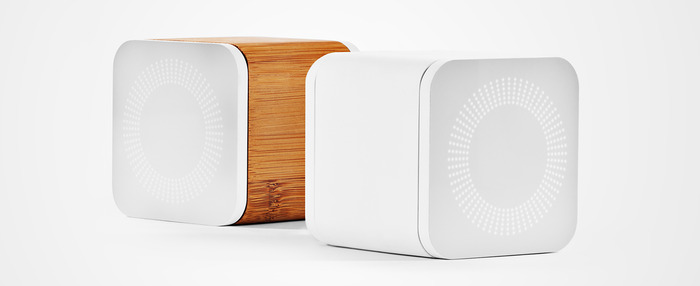
\includegraphics[width=0.90\textwidth,natwidth=610,natheight=642]{figs/circleDevice.jpg}
  	\caption{Kickstarter Project: Meet Circle}
  	\label{fig:circle_project}
\end{figure}
\par The prototype of this report is using \gls{rpi} as the same function as Circle's wireless router. And this prototype system has server side back-end to store client and administrator user database. There are android and \gls{ios} applications both work with the internet control system in this project.
\par At application side, the prototype application of this report will have the same administrator function to approve and block the client internet access request through http request.
\par For the notification function of the system, the project of this report has the similar idea with another kickstarter project 'NINJA SPHERE'\cite{ninja_sphere}. The idea of NINJA SPHERE is to make the next generation control of your environment with accurate in-home location data and a gesture control interface. Although the project of this report will not cover the advanced way to control the environment of the residential area only the internet access control of the residential area, the idea is still the same to use mobile application to communicate with the other device and even get notification from other device in the same wireless network area. 
\par The notification of the client request in this project will be sent as notification E-mail. It makes the administrator get updated request information from the internet access control system.

\section{Scope}
\par The first part of this project will be using the \gls{rpi} device and the code script from previous student master project report\cite{TorgeirMR} and previous student Github repository\cite{TorgierGit} to set up the internet access control system working.Because the \gls{rpi} device and \gls{sd} card  got from the previous student are without any code and configuration, they should be configured with the reference of previous student master project report.
\par The second part of this project will be setting up the central management server on the test domain 'apc.item.ntnu.no'(129.241.200.170)  from \gls{item} department of \gls{ntnu}. The work of this report will cover some security concern improvement and some new notification mechanism implement on the remote central management server.And the database structure of the system stored on the remote server would be changed according to the new functionality of the improved internet access control system.
\par The third part of this project will be implementation of the \gls{ios} application intended for end-user to manage and control clients’ internet access. The application would be implemented under the \gls{ios} 7 \gls{sdk} and Xcode\cite{xcode} 5.0 \gls{ide} on the \gls{macos} 10.8.5 working environment. Since there will be some changes for the central management server, then the android application need to be modified to work with the new back-end server. The changes will be made under \gls{adt}\cite{adt} 22.3.0 \gls{ide}. These two platform application will be tested against central management server and \gls{rpi} device to make sure all the basic administrator function working well.
\par The fourth part of this project will be research about how to make the current internet control system more safe and how to implement more advanced internet control function in the current internet control system. The research would be based on articles and some demo testing script using in the current working internet control system.

\section{Report Structure}
\par In the System Description chapter, it will cover the general information about the previous internet access control system and the improvement form this report project to the current system. In this chapter, some background knowledge of the previous master project\cite{TorgeirMR} would be mentioned as well.
\par In the \gls{rpi} Setting chapter,the main content about the progress to set up \gls{rpi} internet access control will be presented. Some related modification for previous master project would be mentioned in the chapter. And some background research would be including in this chapter to analyze the performance of the current internet access control system
\par In the Central Management Server Improvement chapter would have some detail improved code snippet to be discussed why the previous prototype project need to be improved in this way. And it will show database structure changes on the back-end server as well.
\par In the Mobile Application Development chapter, it will present the basic working process of the application development for this prototype project and some test case to work with the other system components in this internet access control system. The main content of this chapter would be about \gls{ios} application development, but also it will have some modification explanation for android application.
\par In the System Testing chapter, it will show the feedback and analysis from the testing of the prototype project. The analysis will have some future improvement suggestion for later work since there are not enough time to implement the solution to some testing cases.
\par In the Future Work chapter, it will present some better solution for current project to do the internet access control which can not be implement within such short period of this project working time. And there will be some exploring point for the project based on the research of the technical articles.
%% include here the other chapters
\chapter{System Description}
\label{chp:system_description}

\section{Existing Internet Access Control System}
\par This project is based on the existing internet access control system. The existing system provides a manged service for the administrator of the system. The Fgiure \ref{fig:presystem} shows the architecture of the existing system. In this system, the manageable residential access point is \gls{rpi} which has the function as wireless access point and router. The working principle of manipulating iptalbes on \gls{rpi} to give connected devices authenticated \gls{ip} address will not be covered in this report because this project uses same principle of previous master project \cite{TorgeirMR} and the main focus of this project is not system on \gls{rpi}. The setting progress and changes of \gls{rpi} will be covered in the chapter \ref{chp:rpi}. The management server in this architecture is host on the remote server to communicate with the other component in the system. It stores system database and provides \gls{http} communication interfaces. The mobile management application and web management application(not implemented yet) have the same function in the system which is allowed administrator to manage and control the whole system in more mobile and flexible way. The applications for mobile platform covers \gls{ios} and android mobile operating system, since they are main two mobile operating system in the current smart phone shared market.Due to the time limit of this project, the web application development will not be covered in this report although it is easier to make and the working process is the same as other tow platform application. The main function of the mobile applications is to manage the client user internet access request. More detail about it will be covered in the chapter \ref{chp:mobile_app}.
\begin{figure}
	\centering
    	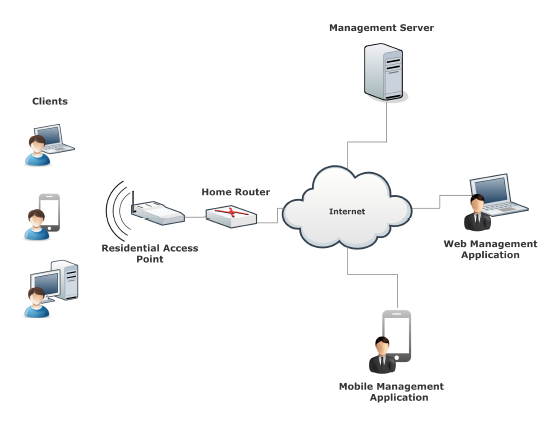
\includegraphics[width=0.80\textwidth,natwidth=610,natheight=642]{figs/presystem.png}
  	\caption{Existing System Architecture}
  	\label{fig:presystem}
\end{figure}

\section{Improvement of Existing System}
\par According to the master project report \cite{TorgeirMR}, there are several function requirements mentioned in that report. In this project, the improvement functions of the system are shown in the Table \ref{tab:improve_system_func}.
\begin{table}
\caption{\label{tab:improve_system_func}: Improvement Functions for System}
\centering
\begin{tabular}{| c | p{4cm} | p{6cm} | l |}
\hline
 No. & Title & Improvement Function & Importance \\ \hline
 1 & Block Internet Access & The residential access point can block clients internet access base on MAC and forbid the \gls{ip} address request & High \\
 2 & Bug Fixed for static \gls{ip} lease & Bug found in the report with wrong script format in static \gls{ip} lease for residential access point & High \\
 3 & Bug Fixed for Missing script & Bug found in the report without essential script file & High \\
 4 & Broken \gls{sd} card changed & Changed broken \gls{sd} card in the project & High \\ \hline
 5 & Security Log on service & Implement security log on mechanism for mobile log on request & High \\
 6 & Complete Authenticate Log on service & Complete implementation of authenticate log on by user-name and password & High \\
 7 & Separate working protocol & Separate client request protocol and mobile management application working protocol on central management server & Medium \\
 8 & Set up Database Management Tool & Set up phpmyadmin\cite{phpmyadmin} to manage database on the central management server & High \\
 9 & E-mail Notification Mechanism & Implement E-mail notification mechanism on central management server to notify the client user internet access request & High \\ \hline
 10 & Security Log on & Implement security log on function on both android and \gls{ios} mobile application & High \\
 11 & Approve and Block Internet access & \gls{ios} Mobile Application can approve and block the client internet access request & High \\
 12 & Real-time update & \gls{ios} Mobile Application can real-time update all the client internet access request & Medium \\ \hline
\end{tabular} 
\end{table}

\section{Analysis of System}
\par The system is based on client-server model \cite{csmodel}, which is a distributed application structure in computing that partitions tasks or workloads between the providers of a resource or service, called servers, and service requesters, called clients. Since in the internet access system, the request client users connect with the residential access point (in this project will be \gls{rpi}), so it is better for the service to provide client-server model communication between different client users and residential access point. 
\par Moreover, there will be different residential access point from different residential areas to communicate with the same service provider (central management server) since the central management server will provide the server back-end service and store the database with information for administrator authentication , different residential \gls{macaddress} address and other necessary service data. The main database of the system should be able to be managed and modified by the administrators. Then the client-server model also would suit into this scenario.
\par According to the communication between mobile application clients and central management server, the client-server model of this architecture is better for central management server to return the response of the \gls{http} request and manage the whole service of the system.
\par More detail about the different components in system architecture would be covered in the individual chapter \ref{chp:rpi}, chapter \ref{chp:central_server} and chapter \ref{chp:mobile_app}.
\par Because there is no running system from previous student master project when this project begin, the performance between previous system and current improvement system would not be compared in this report. However, different improvement of the internet access system would be discussed in the later chapters. And all improvement functions would be only based on the master project report\cite{TorgeirMR}.

\begin{figure}
	\centering
    	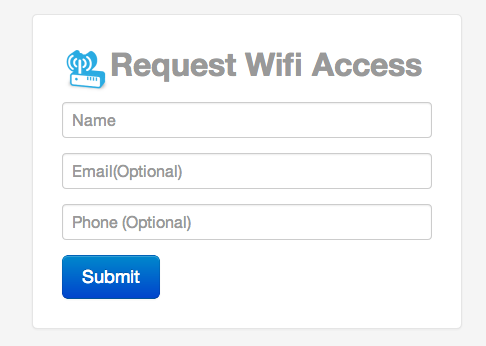
\includegraphics[width=0.60\textwidth,natwidth=610,natheight=642]{figs/wifi_request_page.png}
  	\caption{Request Client User Web Request Page}
  	\label{fig:wifi_request_page}
\end{figure}

\section{User Case}
\par Normal user case for this prototype system will be discussed in this section. There are two children in Adam's family. One is 19-year-old daughter Stella and the other is 15-year-old son Aslak. Usually Adam and his wife Eva live with their younger son, they are using the same wireless network based on internet access control system in their house. However, Aslak likes to play online game too much and sleep very late. Then everyday around 2200, Adam will use his WifiAccess Manager application on his iPhone to block his son's computer internet access to make sure Aslak could sleep at the acceptable time everyday. Some weekend, his daughter come back to their house to enjoy the weekend with them. Stella will make her computer and mobile phone connect with the wireless network, then she use the browser to type any domain name in the address bar, she will be redirected to the same central management server to request internet access like the Figure \ref{fig:wifi_request_page}. Then she just type her name for the current device to make request. After she made request, there will be a notification e-mail send to Adam's phone since his administrator user on the WifiAccess Manager application is registered with this e-mail address. Then Adam will use the ios application to approve this request, after that his daughter can connect with the internet this weekend.

\par More working process will be discussed in the Chapter \ref{chp:system_test}. There will be more detail system testing result in that Chapter.
\chapter{Raspberry Pi Setting}
\label{chp:rpi}
\chapter{Central Management Server Improvement}
\label{chp:central_server}
\chapter{Mobile Application Development}
\label{chp:mobile_app}

\par The source code of \gls{ios} application is on the Github public repository (\url{https://github.com/br1anchen/WifiAccessManager_IOS}). The \gls{ios} project is developed under \gls{macos} 10.8.5 by Xcode 5.0.1 using \gls{ios} 7 \gls{sdk}. The programming language used in this application is Objective-C\cite{objc}, it is a general-purpose, object-oriented programming language that adds Smalltalk-style messaging to the C programming language. It is the main programming language used by Apple for the OS X and iOS operating systems and their respective APIs, Cocoa and Cocoa Touch.The improved Android application's source code is also on the Github public repository \url{https://github.com/br1anchen/WifiAccessManager_Android}. It is developed under \gls{macos} 10.8.5 by \gls{adt}.

\section{IOS Wifi Access Manager Application}

\par During the development period of \gls{ios} management application, Apple just released new \gls{ios} \gls{sdk},which is \gls{ios} 7, on all the \gls{ios} devices. And the new Xcode \gls{ide} is upgraded with this new \gls{sdk} library as well. So for this prototype project, \gls{ios} application is developed under these \gls{sdk} scope. Because of the time limit for this project and the main goal of the application is not to provide advanced mobile application, some necessary feature like user interface design will not be considered as high priority in this project. Furthermore, it is simple management application for prototype, it will not include highly advanced software design architecture.

\subsection{SDK Library Using in IOS Wifi Access Manager Application}
\par There are three key \gls{sdk} libraries used in this project. 

\subsubsection{Foundation.framework}
\par The first one is Foundation Framework library \cite{foundationlib},it defines a base layer of Objective-C classes. In addition to providing a set of useful primitive object classes, it introduces several paradigms that define functionality not covered by the Objective-C language. It is designed with these goals in mind:
\begin{itemize}
  \item Provide a small set of basic utility classes.
  \item Make software development easier by introducing consistent conventions for things such as deallocation.
  \item Support Unicode strings, object persistence, and object distribution.
  \item Provide a level of OS independence, to enhance portability.
\end{itemize}
\par Most of the \gls{ios} application is based on this important library because it includes the root object class, classes representing basic data types such as strings and byte arrays, collection classes for storing other objects, classes representing system information such as dates, and classes representing communication ports.

\subsubsection{CoreGraphics.framework}
\par The second library is Core Graphics Framework library \cite{coregraphicslib}. It is a C-based API that is based on the Quartz advanced drawing engine. It provides low-level, lightweight 2D rendering with unmatched output fidelity. You use this framework to handle path-based drawing, transformations, color management, offscreen rendering, patterns, gradients and shadings, image data management, image creation, masking, and PDF document creation, display, and parsing. In this project, the application's request list swiping to approve or block gesture animation is based on this library although this customized user interface component is also based on the other third party class library. The working animation result of this user gesture is shown in Figure \ref{fig:ios_swipe}.

\subsubsection{UIKit.framework}
\par The third \gls{sdk} library used in the project is UIKit Framework library \cite{uikitlib}. It provides the classes needed to construct and manage an application’s user interface for iOS. It provides an application object, event handling, drawing model, windows, views, and controls specifically designed for a touch screen interface. Since mobile applications require very high responsiveness for user interface behavior, this library will provide all these kinds of event to the application logic to handle with. For example, the swipe gesture in this application, it will dispatch an user interface swipe event to the run-time system, and the touch event on the login button will dispatch another touch event to the run-time system as well.

\subsection{Third Party Library Using in IOS Wifi Access Manager Application}

\par Although the native \gls{sdk} \gls{ios} 7 library provided by Apple is quite powerful and convenient to use, there are still some process missing or not good enough to work with. Then third party library provided as open source project is necessary to use in this application.

\subsubsection{UITableViewCell-Swipe-for-Options}
\par In order to make the managing process of the client requests approving or blocking more convenient to use, the similar gesture function using in \gls{ios} 7 Mail App is a good solution for administrator to approve or block a client request in the connect device list by just swiping the corresponding list row and choose the approve or block button to make the management command to server. This open source project,UITableViewCell-Swipe-for-Options\cite{swipe-for-options}, hosted on Github is better choice in this project to replace with the normal UITableViewCell component( which is default table row component in \gls{ios} user interface).

\subsubsection{JSONKit}
\par JSONKit\cite{jsonkit} library is a very high performance Objective-c \gls{json} Library. Although in \gls{ios} 7 \gls{sdk}, it provides the simple \gls{json} parsing and serializing function. But it is limited with complexity of the \gls{json} object needed to be parsed or serialized. In this project, the \gls{json} object using during the communication between mobile client and server is quite complicated data structure object, then by using this third party \gls{json} library is easier for developer to program the application. Moreover, the performance of the JSONKit to parse data to \gls{json} object or serialize the \gls{json} object to Objective-c object is better than any \gls{json} framework in \gls{ios} application development scope according to the documentation of JSONKit library.

\subsubsection{Base64}
\par Base64\cite{base64lib} library is a set of categories that provide methods to encode and decode data as a base-64-encoded string. Because of the security login mechanism is implemented on the central management server, it is required for \gls{ios} mobile application to have Base64 encoding process. The third party Base64 library is introduced for this reason.

\subsection{Structure of IOS Wifi Access Manager Application}

\subsubsection{Story Board}

\begin{figure}
	\centering
    	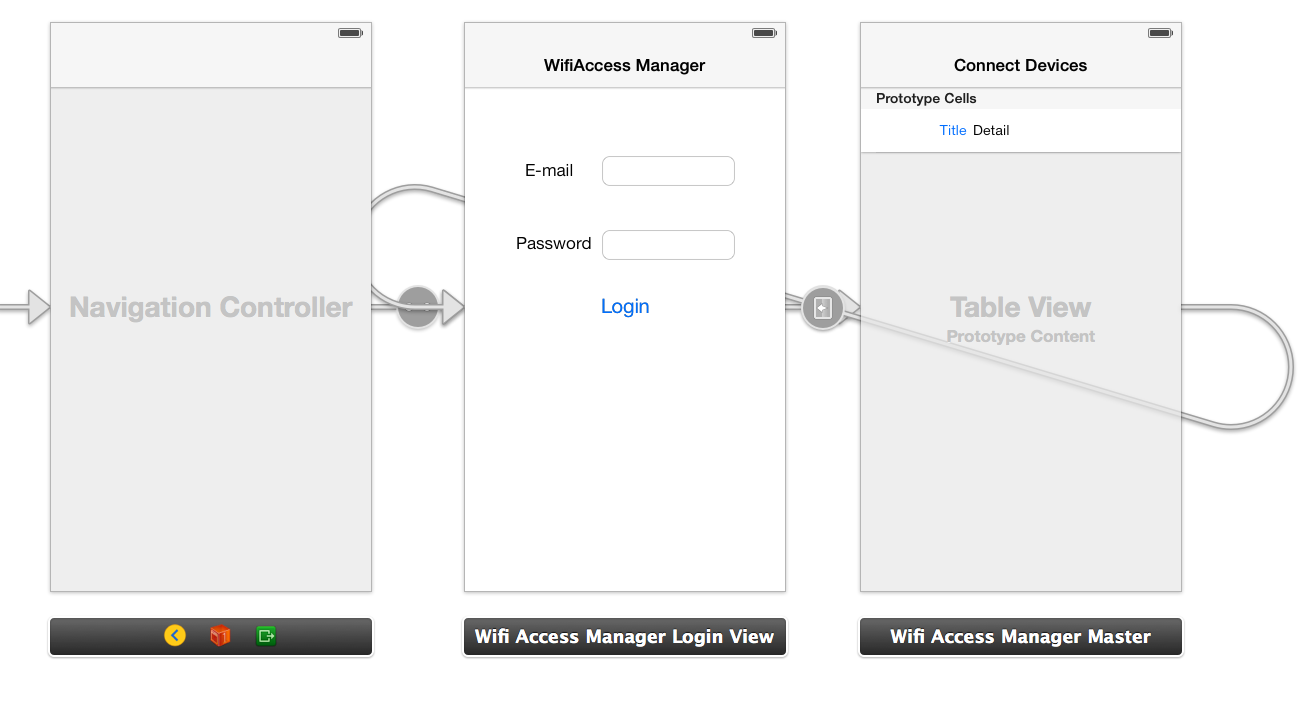
\includegraphics[width=0.80\textwidth,natwidth=610,natheight=642]{figs/ios_app_storyboard.png}
  	\caption{IOS Mobile Application Story Board Design}
  	\label{fig:ios_storyboard}
\end{figure}

\par Storyboard\cite{xcode_storyboard} is a visual representation of the user interface of an iOS application, showing screens of content and the connections between those screens. A storyboard is composed of a sequence of scenes, each of which represents a view controller and its views; scenes are connected by segue objects, which represent a transition between two view controllers.

\par Xcode provides a visual editor for storyboards, where developer can lay out and design the user interface of the application by adding views such as buttons, table views, and text views onto scenes. In addition, a storyboard enables developer to connect a view to its controller object, and to manage the transfer of data between view controllers. Using storyboards is the recommended way to design the user interface of the application because they enable developer to visualize the appearance and flow of your user interface on one canvas. Story board is used to simplify the structure of this application.

\par The story board design of the \gls{ios} application is shown in Figure \ref{fig:ios_storyboard}. There are only two visible view in the story board, which are Wifi Access Manager Login View and Wifi Access Manager Master View. The controller to push or pop other user interface view to the font scene is navigation controller. Wifi Access Manager Login View is the place for administrator of the internet access control system to login the mobile application. And the Wifi Access Manager Master view is a subview of the UITableView(the user interface view class in \gls{ios}), it consists a list of the connected devices in the residential wireless network with status of each device's access request.

\subsubsection{View Controllers}
\par Since there are two views in the application, each of them has their own view controller to handle the user interface event with the corresponding application logic function. 
\par The view controller for Login View shown in Figure \ref{fig:ios_login_page} and Figure \ref{fig:ios_login_process} is WifiAccessManagerLoginViewController. The userLogin function (the main application logic function in WifiAccessManagerLoginView) is display in the Code Snippet \ref{code:ios_userlogin}. In this function, it takes the values from the user interface input as E-mail and password, then use the helper class (HttpRequestUtilities) which will be discussed later in this chapter to make the \gls{http} post request to the central management server for checking the user authentication. If login is successful it will use the story board 'performSegueWithIdentifier' function to get the corresponding segue by the name 'afterLogin'. The login process is shown in Figure \ref{fig:ios_login_process} After that this segue will be triggered, which is to push the Wifi Access Manager Master view to the font scene. Also the administrator login information will be stored as user profile in this application sandbox folder, it will be used for later multitask switching application process on \gls{ios} from other application to make the user no need to type again to login.

\begin{algorithm}[h]
\floatname{algorithm}{Code Snippet}
  \caption{userLogin function in WifiAccessManagerLoginViewController.m}
  \label{code:ios_userlogin}
  \begin{verbatim}
  
- (IBAction)userLogin:(id)sender {
    self.email = self.email_input.text;
    self.password = self.pwd_input.text;
    
    NSString *loginInfo = 
    		[NSString stringWithFormat:
    			@"WifiAccess Manager:Login:email: %@, pwd: %@",
    			self.email,self.password];
    NSLog(@"%@", loginInfo);
    
    HttpRequestUtilities *httpHelper = [[HttpRequestUtilities alloc] init];
    
    if([httpHelper loginRequest:self.email withPassword:self.password])
    {
        NSLog(@"Login Success.");
        NSUserDefaults *userPref = [NSUserDefaults standardUserDefaults];
        [userPref setValue:self.email forKey:@"Email"];
        [userPref synchronize];
        
        [self performSegueWithIdentifier: @"afterLogin" sender: self];
    }else{
        NSLog(@"Login Failed.");
        UIAlertView *loginAlert = 
        		[[UIAlertView alloc] 
        			initWithTitle:@"Login Failed" 
        			message:@"Please check your user information then login again" 
        			delegate:self 
        			cancelButtonTitle:@"OK" 
        			otherButtonTitles:nil,nil];
        [loginAlert show];
    }
}

 \end{verbatim}
\end{algorithm}

\begin{figure}
	\centering
	\begin{minipage}{0.45\textwidth}
		\centering
    		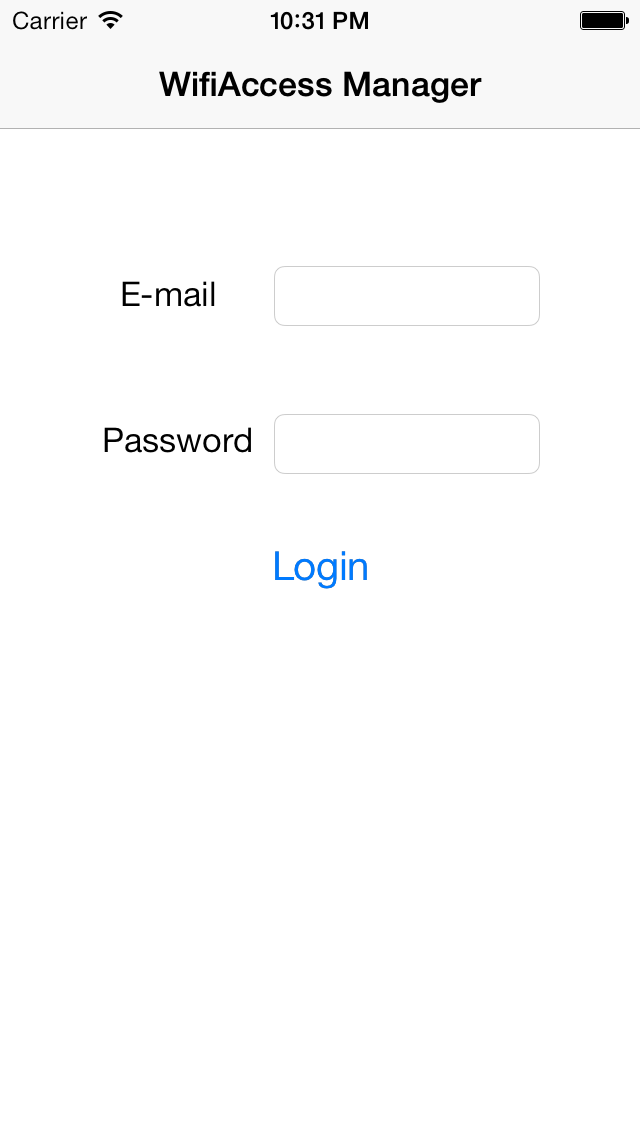
\includegraphics[width=0.6\textwidth,natwidth=610,natheight=642]{figs/ios_app_login_page.png}
  		\caption{IOS Mobile Application Login View}
  		\label{fig:ios_login_page}
  	\end{minipage}
  	\hfill
  	\begin{minipage}{0.45\textwidth}
  		\centering
  		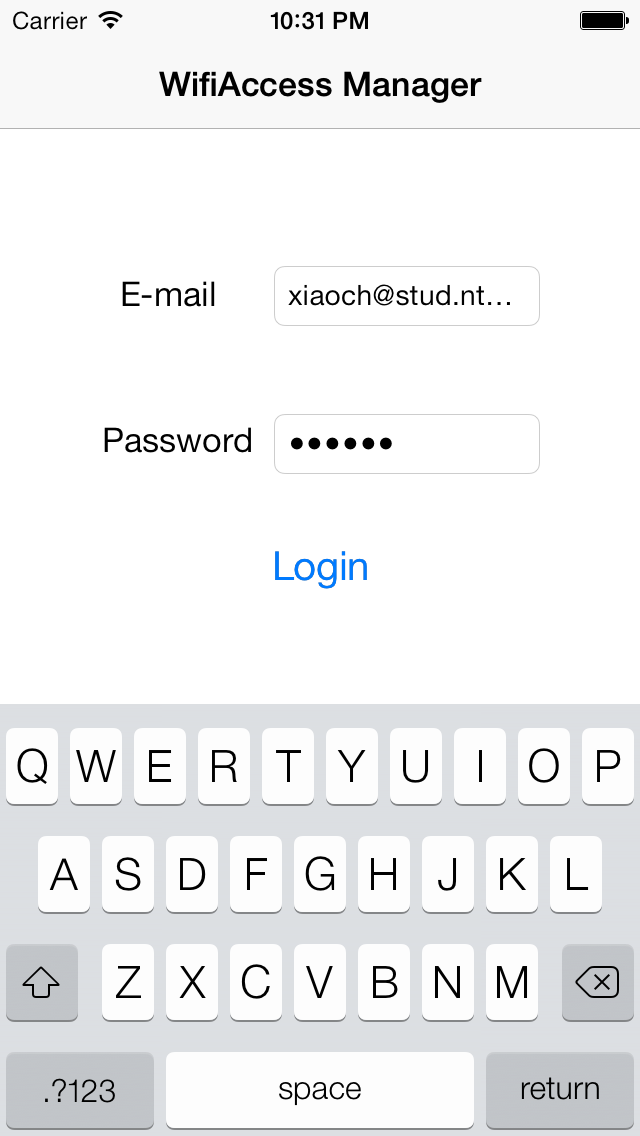
\includegraphics[width=0.6\textwidth,natwidth=610,natheight=642]{figs/ios_app_login_process.png}
  		\caption{IOS Mobile Application Login Process}
  		\label{fig:ios_login_process}
  	\end{minipage}
\end{figure}

\begin{figure}
	\centering
	\begin{minipage}{0.45\textwidth}
  		\centering
  		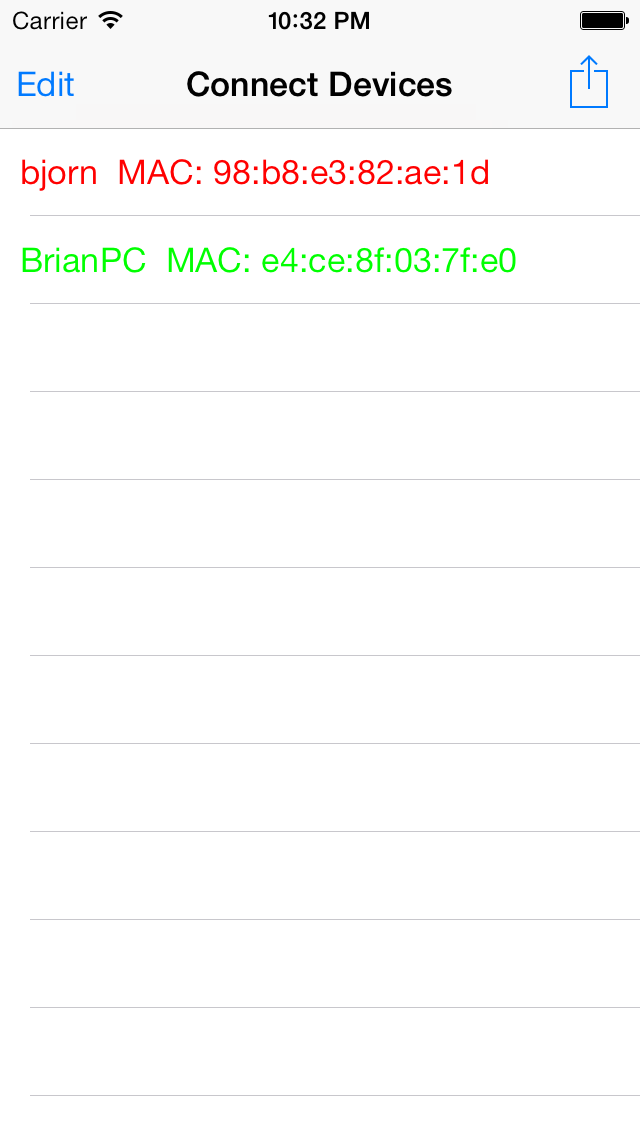
\includegraphics[width=0.6\textwidth,natwidth=610,natheight=642]{figs/ios_app_request_list.png}
  		\caption{IOS Mobile Application Request List View}
  		\label{fig:ios_requests}
  	\end{minipage}
  	\hfill
	\begin{minipage}{0.45\textwidth}
		\centering
    		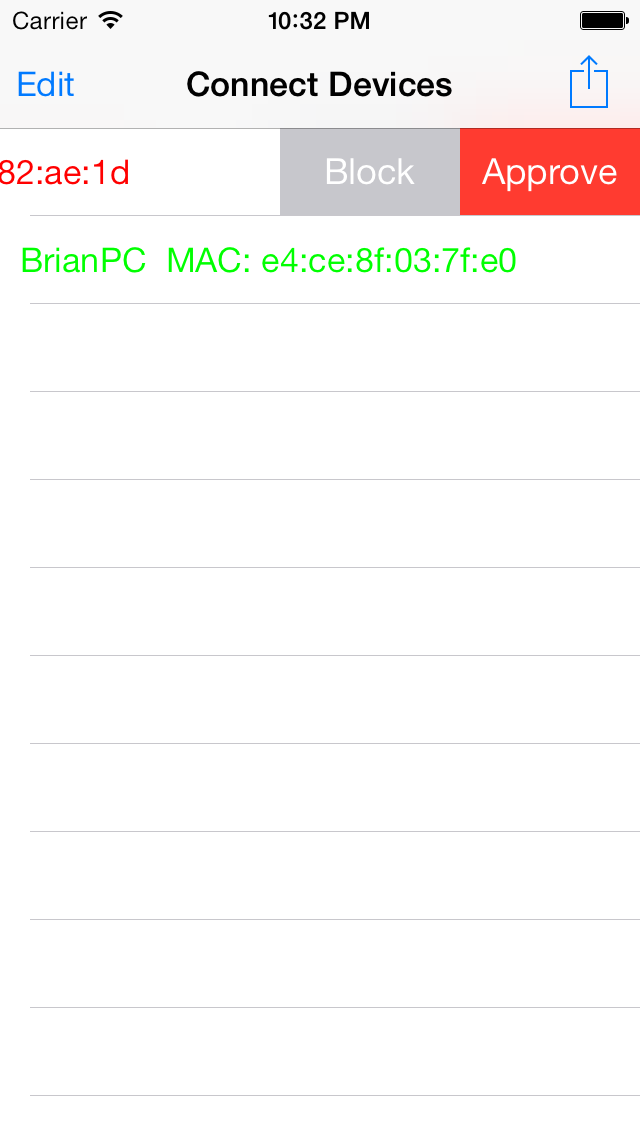
\includegraphics[width=0.6\textwidth,natwidth=610,natheight=642]{figs/ios_app_manage_gesture.png}
  		\caption{IOS Mobile Application Swipe Gesture}
  		\label{fig:ios_swipe}
  	\end{minipage}
\end{figure}

\par The view controller for Wifi Access Manager Master view is more complicated than Wifi Access Manager Login View because it includes a UITableView, swipe gesture function with approving and blocking request function and automatic updating function. Because the view of this view controller is a table view then this view controller is a sub-view controller  class of UITableViewController. It will have the delegate functions from UITableViewController to controll the table view. Moreover it will have the delegate functions from third party library,TLSwipeForOptionsCellDelegate, to make the swipe to options function work on cell components in the table view. The loadTableData function shown in Code Snippet \ref{code:ios_loadtabledata} of Appendix \ref{chp:appendix2}, is the function to get the request lists from the server. It calls the helper class (HttpRequestUtilities) to make the \gls{http} post request to the central management server to get all the requests for the corresponding administrator. Then using the \gls{json} serialization to convert the \gls{json} object array to the objective-c NSMutableArray for displaying in the table view. But since the mechanism of \gls{ios} is to not block the user interface thread all the time, so this load table data will be run as another separate thread, after fetching the data from the server, reloadData function of self.tableView needs to be called to force the table content refresh with the new fetching data. The result after this process is shown in Figure \ref{fig:ios_requests}.

\par The automatic updating function is implemented as a timer repeats with 10 second interval to call the loadTableData function in the application. The implementation code is shown in Code Snippet \ref{code:ios_updatetimer}.

\begin{algorithm}[h]
\floatname{algorithm}{Code Snippet}
  \caption{timer code in WifiAccessManagerMasterViewController.m}
  \label{code:ios_updatetimer}
  \begin{verbatim}
  
    updateTimer = [NSTimer scheduledTimerWithTimeInterval:10 
    							target:self 
    							selector:@selector(loadTableData) 
    							userInfo:nil 
    							repeats:YES];
    [updateTimer fire];
 \end{verbatim}
\end{algorithm}

\begin{figure}
	\centering
	\begin{minipage}{0.45\textwidth}
		\centering
    		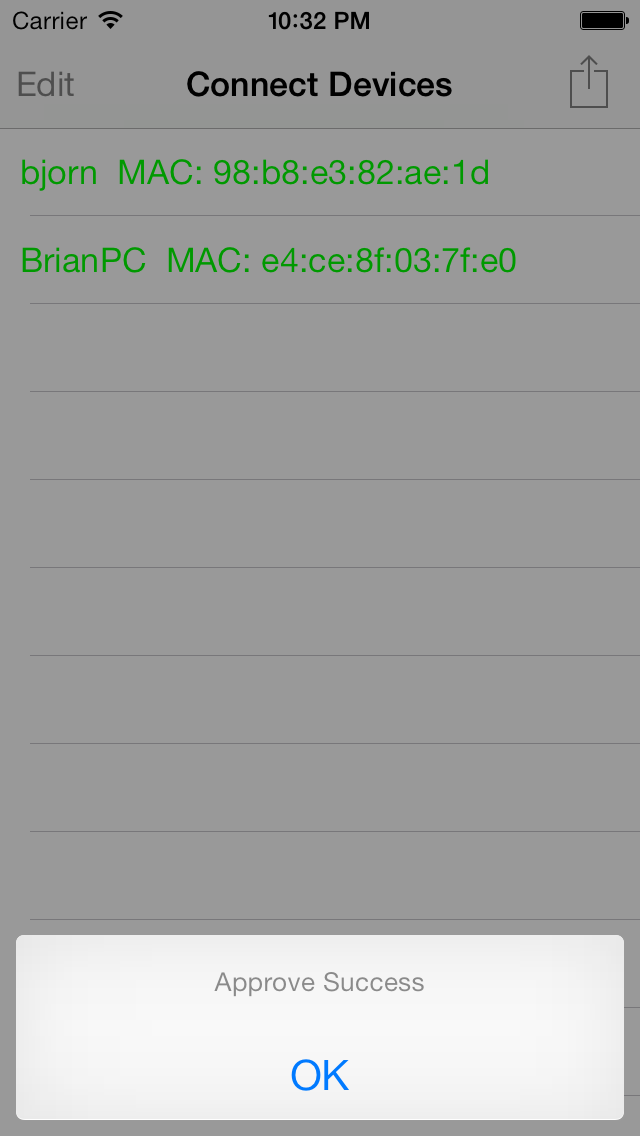
\includegraphics[width=0.45\textwidth,natwidth=610,natheight=642]{figs/ios_app_approve_request.png}
  		\caption{IOS Mobile Application Approve Request Process}
  		\label{fig:ios_approve}
  	\end{minipage}
  	\hfill
  	\begin{minipage}{0.45\textwidth}
  		\centering
		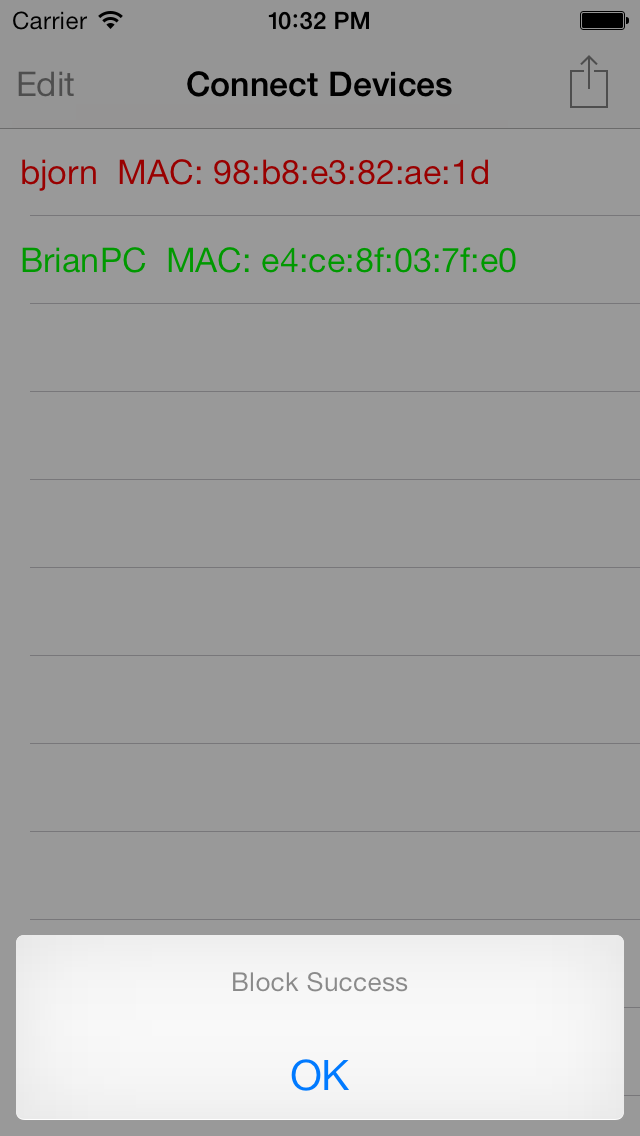
\includegraphics[width=0.45\textwidth,natwidth=610,natheight=642]{figs/ios_app_block_request.png}
  		\caption{IOS Mobile Application Block Device Process}
  		\label{fig:ios_block}
  	\end{minipage}
\end{figure}

\par The approving and blocking process shown in Figure \ref{fig:ios_approve} and Figure \ref{fig:ios_block} is implemented by the similar way in the WifiAccessManagerMasterViewController. In this report, only approving function displayed in Code Snippet \ref{code:ios_approve} of Appendix \ref{chp:appendix2} will be discussed as code sample of these application process. This function is a delegate function from TLSwipeForOptionsCell class, which provides the method to get current select row of the table view to do further application process. The 'cellDidSelectApprove' function shown in Code Snippet \ref{code:ios_approve} of Appendix \ref{chp:appendix2} from this application will get the corresponding data from the current selected row to make the \gls{http} post request to post the changes for the client request status(in this case it is approving the request). Like loadTableData function mentioned before, it is a thread safe process as well, so it is necessary to call the loadTableData to fetch latest data from central management server and then force the table view to refresh the content.

\subsubsection{HttpRequestUtilities}
\par To make the work of development for this application easier, one helper class named as HttpRequestUtilities is made in the project. This class will use other two third party library(JSONKit,Base64) to handle all the \gls{http} request to the server. There are three different \gls{http} request in the application. They are shown as Code Snippet \ref{code:ios_http_login}, Code Snippet \ref{code:ios_http_getrequests} and Code Snippet \ref{code:ios_http_postclient} in the Appendix \ref{chp:appendix2}. They are main \gls{http} communication between the mobile application client and central management server.All of them are quite similar, the function sets an \gls{url} with the corresponding address string, then creates a  NSMutableURLRequest object to set all the corresponding information data in \gls{http} request header or body, at last makes the NSURLConnection with the central server to get the response back.

\section{Improvement for Android Application}
\par Because of the security login mechanism on the central management server, there will be some changes on Android Application as well. By using the android.util.Base64 library, the encoding user name and password process is implemented. In the previous master project, there is no login parameter for password, so it needs to be added for Android Application. The main changes is shown in the Code Snippet \ref{code:android_login}.

\begin{algorithm}[h]
\floatname{algorithm}{Code Snippet}
  \caption{login changes on Android Application}
  \label{code:android_login}
  \begin{verbatim}
  
Map<String, String> loginParams = new HashMap<String, String>();
loginParams.put("email", 
		Base64.encodeToString(mEmail.getBytes(), Base64.DEFAULT));
loginParams.put("password", 
		Base64.encodeToString(mPassword.getBytes(), Base64.DEFAULT));
 \end{verbatim}
\end{algorithm} 
\chapter{System Testing}
\label{chp:system_test}
\par There are three main components in this project system. There are \gls{rpi} residential access point, central management server and mobile application. So in this chapter test process will cover these three parts of the system.

\section{Testing on \gls{rpi}}
\par To test the system on \gls{rpi}, the working place shown in Figure \ref{fig:rpi_test} needs to be set up. Since the \gls{rpi} using in this project has only two bulit \gls{usb} port, one is taken by Wireless-G \gls{usb} Dongle. Then it is necessary to use an \gls{usb} hub to provide two more \gls{usb} port for keyboard and mouse to connect with. It is important that the \gls{usb} hub connected with \gls{rpi} is not require too high power voltage from \gls{rpi} because the power voltage is quite limited on \gls{rpi} board. Furthermore, the power cable of \gls{rpi} need to be check if it can be used for higher voltage power adapter because some time the normal data transition micro-usb cable is not enough to power up the \gls{rpi} device. To make the test and development of this project convenient, a \gls{hdmi} cable is used for \gls{rpi} to output display signal to the monitor. At last, the ethernet cable is required to give the \gls{rpi} access to the internet.

\begin{figure}
	\centering
    	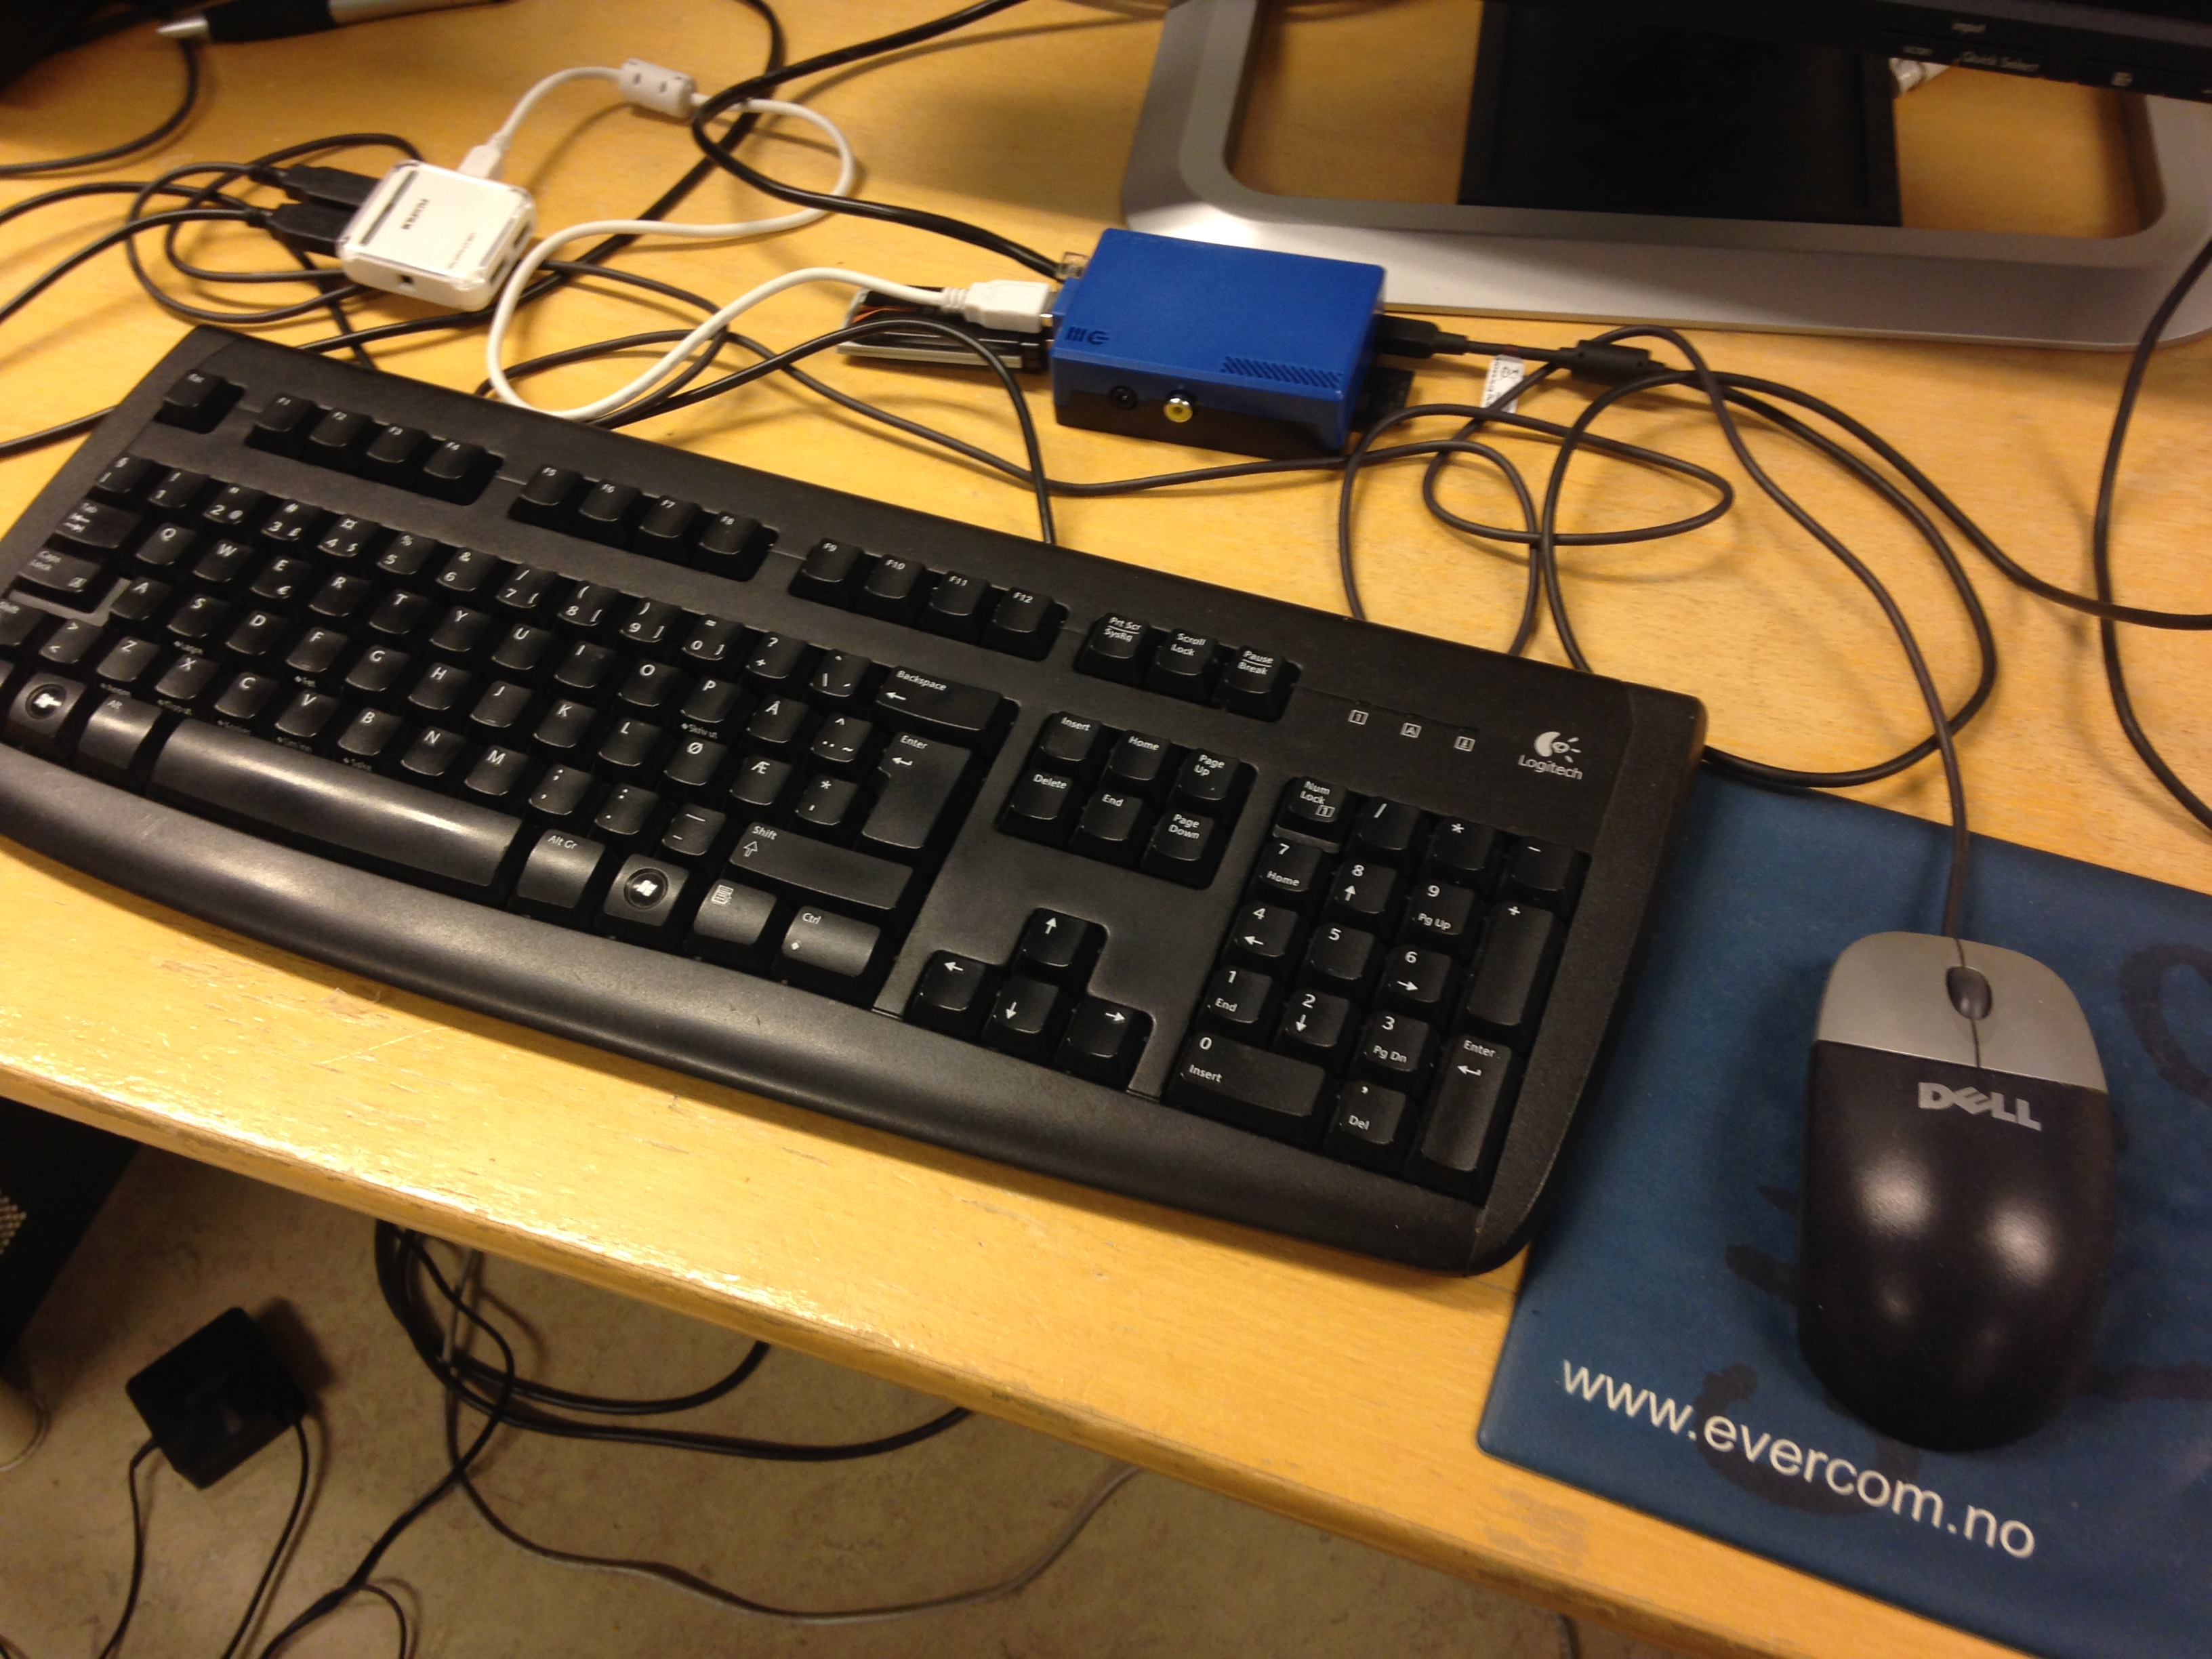
\includegraphics[width=0.80\textwidth,natwidth=610,natheight=642]{figs/rpi_test.JPG}
  	\caption{RPI Test Working Place}
  	\label{fig:rpi_test}
\end{figure}

\par The two python scripts partly shown in Code Snippet \ref{code:configserver_py} in Appendix \ref{chp:appendix} and on the Github repository \url{https://github.com/br1anchen/WifiAccess_RPIConfigurationServer/blob/master/transproxy.py} should be executed and keep running on \gls{rpi}. The full version of source code can be found on the Github repository \url{https://github.com/br1anchen/WifiAccess_RPIConfigurationServer}. The method of testing access point system on \gls{rpi} is to change the database of the client table (shown in the Figure \ref{fig:database_request}) on the central management server. The columns, 'json\_permission' and 'update\_flag' in the client table need to be changed to triggered the changing access right process for the corresponding client on the \gls{rpi}. For example, in the Figure \ref{fig:database_request}, the client 'BrianPC' is with the 'json\_permission' value '\{"permissions":\{"access":\{"allow":true\}\}\}' and the 'update\_flag' value '1'. It means that this client is approved by administrator and need to be updated its \gls{ip} address lease on the \gls{rpi} residential access point. For the test purpose, the 'json\_permission' value can be changed as '\{"permissions":\{"access":\{"allow":false\}\}\}' and keep the 'update\_flag' value still as '1'. Then the \gls{rpi} will know that this device is not allowed to access the residential network anymore, will make the blocking process for it.

\par The feedback of testing on \gls{rpi} shows that it is not easy for normal user to set up this internet access control system. And since the running process log only can be shown on external monitor by \gls{rpi}, the running scripts on the \gls{rpi} has no way to notify the normal user if there is error or failure of the running process. The suggested solution of this feedback will be discussed in Chapter \ref{chp:future_work}.

\begin{figure}
	\centering
    	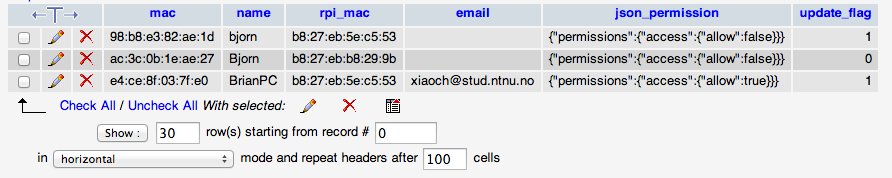
\includegraphics[width=0.80\textwidth,natwidth=610,natheight=642]{figs/database_request.png}
  	\caption{Client Database Table on Central Management Server}
  	\label{fig:database_request}
\end{figure}

\section{Testing on Central Management Server}
\par Because in this project, we make the improvement for login mechanism and E-mail notification for Central Management Server.So the test will be done for these two main feature of the Central Management Server.

\subsection{Login Mechanism Testing}
\par The login process communication between mobile application and central management server is \gls{http} post request with some user information on the request payload. The test for this feature will use a Chrome browser extension application called Advanced Rest Client to demonstrate the \gls{http} post request from the mobile application. The concept of Advanced Rest Client application is based on cURL\cite{curl} command, which is a computer software project providing a library and command-line tool for transferring data using various protocols. The working process to test login mechanism on central management server is shown in the Figure \ref{fig:restclient_test}. Because the user information data need to be encoded by Base64, then some online Base64 encoder web service is also used in this project for testing quite often, such as \url{http://www.base64encode.org/}. In Figure \ref{fig:restclient_test}, the use of Advanced Rest Client application is quite clear that it allows user to edit the value in the \gls{http} request header and payload. It helps the development and testing a lot.
\begin{figure}
	\centering
    	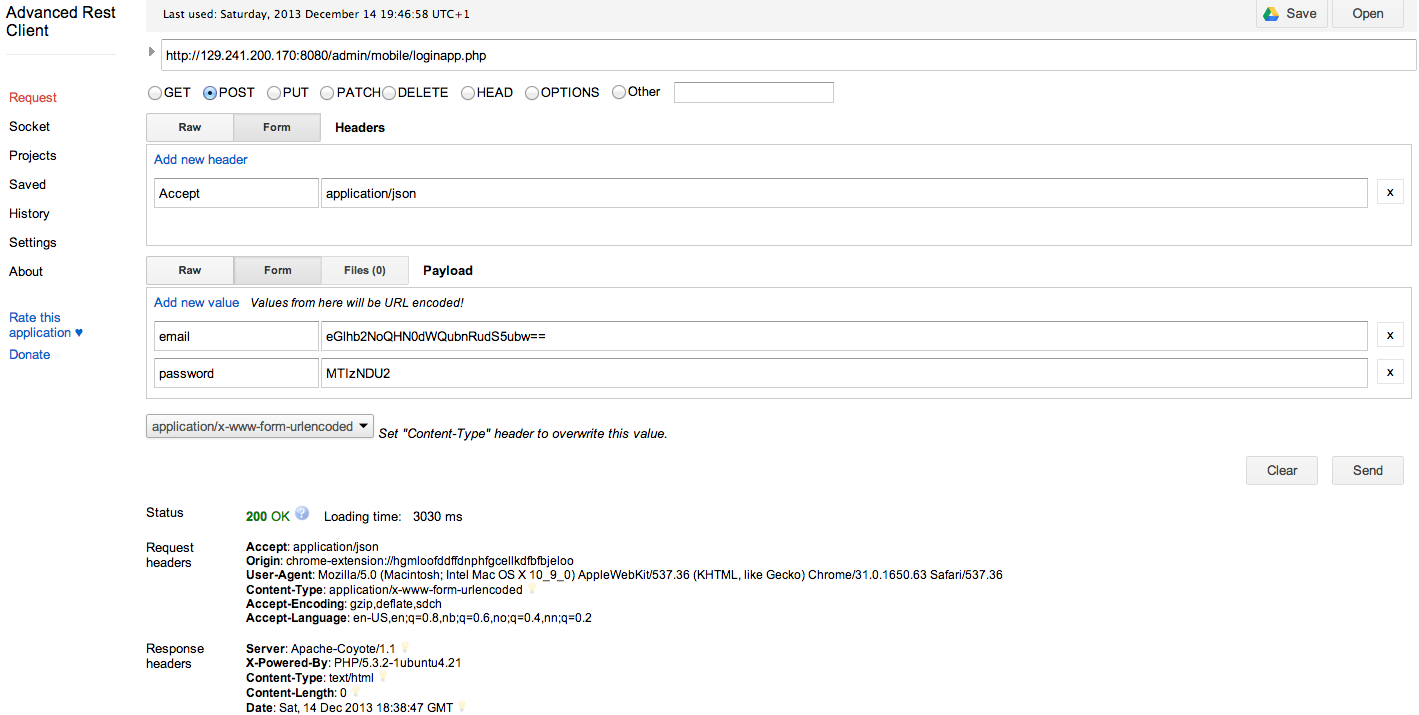
\includegraphics[width=0.80\textwidth,natwidth=610,natheight=642]{figs/restclient_test.png}
  	\caption{Advanced Rest Client Chrome Extension App for Central Management Server Test}
  	\label{fig:restclient_test}
\end{figure}

\par For testing the login mechanism on the central management server, the changing of the user information(for mobile manager client) database is also necessary. The Figure \ref{fig:database_user} is the administrator page of phpmyadmin for User database table on the central management server. By using phpmyadmin, the work to observe the changes of database and modify the database content or structure is much more easier than the previous master project.
\par The feedback of testing for login mechanism shows that it is a good solution to make the communication between mobile client and server more security than previous master project.And it makes the central management server hide behind the font side of the communication channel.
\begin{figure}
	\centering
    	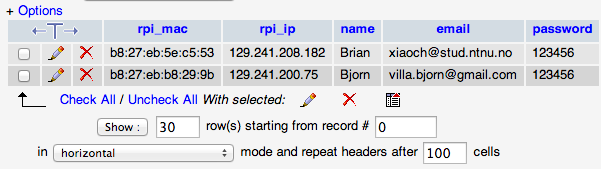
\includegraphics[width=0.80\textwidth,natwidth=610,natheight=642]{figs/database_user.png}
  	\caption{User Database Table on Central Management Server}
  	\label{fig:database_user}
\end{figure}

\subsection{E-mail notification}
\par To test the e-mail notification process of central management server is quite easy because the client request page shown in Figure \ref{fig:wifi_request_page} described in Chapter \ref{chp:system_description} can be used multiple times on one connected device in the network. It is reasonable since if the user is allowed in the residential network, then it should allow them to get the request result no matter it is approving or blocking. Then every time the client make the access request to the central management server, corresponding administrator need be notified by the E-mail from system. Although the weakness of the Brute-force attack will happen because of this process way, but by fixing the server work load case it should be handled quite well, this case will be more discussed in the Chapter \ref{chp:future_work} based on the feedback from the testing.
\par Through the testing of E-mail notification mechanism, the responsible administrator will get E-mail from the system E-mail address like the mail shown in Figure \ref{fig:request_note_mail}.
\begin{figure}
	\centering
    	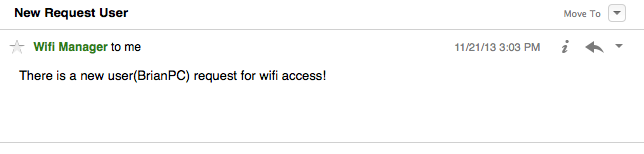
\includegraphics[width=0.80\textwidth,natwidth=610,natheight=642]{figs/request_note_mail.png}
  	\caption{Notification E-mail for Administrator}
  	\label{fig:request_note_mail}
\end{figure}
\par The feedback of this test shows that it is nice way to replace with the normal push notification function since there is no Apple developer account available in this prototype project.

\section{Testing on Mobile Application}
\par Because the simplicity of the mobile application, there is no test framework using during the development.The testing on mobile application is more focus on manually test for all the user behavior function on the mobile application. In this project, testing is on \gls{ios} mobile application. Since the time of development of this application is during the transition from old mobile operating system to new mobile operating system by Apple, more tests for application performance on different \gls{ios} platform.
\par Because of the limitation of different \gls{ios} devices with different versions of \gls{ios}, testing of mobile application has to be done on the simulator to get test result. Xcode \gls{ide} provides different simulators running different versions of \gls{ios} operating system. It also provides different versions of mobile \gls{cpu} like 32-bit and 64-bit on different simulators. The functionality testing is working on different simulators with different assert. According the result of testing, the \gls{ios} Wifi Manager mobile application is working well on all different kinds of simulators. The performance result of different simulators test shows that all the test have almost the same performance on all kinds of simulators. The reason for that, it is mainly because of the simplicity of the application and not physical devices running different versions of \gls{ios}.
\chapter{Future Work}
\label{chp:future_work}

\par According the work progress of this report project and feedback from tests in the Chapter \ref{chp:system_test}, there are several key features need to be considered as the future work for current internet access control system. Since there are no tests for these suggestion to the current system, some of the suggestion of the future could be hard to implement with. However, the considering fields of these approach would be more important than the implementation solutions in this Chapter.

\section{Real-time Request Handle on Central Management Server}
\par On the current central management server of the internet access control system, the back-end web service is implemented by \gls{php}. And to get the update request status information from the server is achieved by a repeated timer to send \gls{http} post request. These facts make the request status information in the system is not real-time updated and also there will be too many useless \gls{http} requests between the \gls{rpi} and central management server. These weakness is not so magnificent when there is only one residential network for the central management server to host web service. But the reason to have a central management server is to have the ability to host one service to serve different residential networks with the different \gls{rpi} residential network access points. Then the work load problem will happen in current system, and also the weakness of the not real-time data will cause much more delay of request information for the end user.
\par From the research about real-time web service, some web technology framework focus on real-time communication like Node.Js\cite{nodejs} could be a better solution to host web service and \gls{api} for mobile application in this system.Node.js is a platform built on Chrome's JavaScript run-time for easily building fast, scalable network applications. Node.js uses an event-driven, non-blocking I/O model that makes it lightweight and efficient, perfect for data-intensive real-time applications that run across distributed devices. Research article(Performance analysis among Node.Js and other web server)\cite{jsconf2010} shows that Node.Js is faster than apache\&php based web server on handling with many small dynamic requests(which is the post request from \gls{rpi}), so the performance of both raspberry pi client and mobile application client to pull and push data from server will be better.

\section{Website Filtering Block Solution}
\par The focus scope of this internet access control system is on residential use and parental control. Then the function of filtering website as white list and black list is necessary for this system. Since the basic concept of current system is to manipulate the \gls{ip} table, then using some specific iptalbes command to block website is a proper solution. For example, the command in Code Snippet \ref{code:iptables_block} tested in the current system is working for blocking website purpose. Then there could be a blocking website mechanism in the current system to let the administrator make a black list for the blocking website. Every time the running scripts on the \gls{rpi} get this list from the central management server, it will use the same command in Code Snippet \ref{code:iptables_block}
 to block the websites.
\begin{algorithm}[h]
\floatname{algorithm}{Code Snippet}
  \caption{Block Website Command in iptables}
  \label{code:iptables_block}
  \begin{verbatim}
  iptables -I FORWARD  -m string --string "facebook.com" 
  					--algo bm --from 1 --to 600 -j REJECT
 \end{verbatim}
\end{algorithm}

\par However, blocking sites with iptables rules is not a good idea, mainly because iptables (as most firewalls) deals with the \gls{ip} addresses, but the relationship between a site and its \gls{ip} addresses is rather loose.

\par One site can have many \gls{ip} addresses, which can be changed rather frequently. Once iptables rules are created, even if you specify a site's name as part of a rule, the first \gls{ip} address at that moment is used. If site's address changes, your iptables rules will be out of date. One \gls{ip} address can host many sites (and it happens often). This will only get more frequent, because of the \gls{ip} address scarcity. Then if you block an \gls{ip} address, you block all sites hosted on it.

\par So it is better to use other solution than manipulating the iptables although in current system it is hard to implement because the structure of the current system is based on manipulating the iptables rules. The other possible solution will be discussed in next section.

\section{Other Solution than Iptables}
\par The main method used in current system on \gls{rpi} is to manipulate the iptables rules. But it is not safe since the access right is only based on whether the \gls{ip} address is authenticated or not. The other possible solution to achieve the same goal of internet access control should be considered. For example, installing a transparent \gls{http} proxy will achieve that. There is a project named 'Transparent Proxy with Linux and Squid mini'\cite{transparentproxy} is quite promising for this case. Once the system has a transparent proxy, arbitrary rules can be added to it to block specific sites, it even does not need to use the caching feature of squid.There are other ways to handle site blocking like firewalls, proxies, etc. They should be more considered if this system need to be used in more practical field.

\section{Request Security}
\par As mentioned in Chapter \ref{chp:central_server}, the login mechanism in the system is safe \gls{http} request because it is using Base64 encryption for the user login information. However, other \gls{http} requests in the system are still based on string parameter in request which can be weakness of the system security. Then the solution to encrypted these request parameter is also necessary, otherwise to set up all the \gls{http} request based on \gls{https} communication protocol would be another choice.

\section{\gls{rpi} system distribution}
\par The main purpose of the \gls{rpi} in this residential internet access network is to set up and work stand alone, no need to be configured later on. If this product need to be focus on commercial market, then these two running scripts on the \gls{rpi} need to start running when \gls{rpi} boot up. The solution in this article 'Running A Python Script At Boot Using Cron'\cite{runatboot} could be a good solution for this approach. It use an application called Cron to be a job scheduler that allows the system to perform tasks at defined times or intervals. It is a very powerful tool and useful in lots of situations. \gls{rpi} can use it to run commands or in this case, two Python scripts when it boots.
\par Then the \gls{rpi} in the system just needs to be powered up, all the running scripts will be executed when it boots, and no need for customer to configure it to start the service.

\renewcommand*{\bibname}{References}
\bibliographystyle{alpha}
\bibliography{main}

\appendix
\addtocontents{toc}{%
  \protect\vspace{1em}% 
  \protect\noindent \bfseries \appendixtocname\protect\par
  \protect\vspace{-.5em}%
 }
 \renewcommand{\chaptername}{\appendixname}
%% include below possible appendices (chapters)
\begin{appendices}
\chapter{Appendix}
\label{chp:appendix}
\section{RPI Residential Access Point Scripts}

\begin{algorithm}[h]
\floatname{algorithm}{Code Snippet}
  \caption{network interface configuration file}
  \label{code:network_interface}
  \begin{verbatim}
  
auto lo

iface lo inet loopback
iface eth0 inet dhcp

allow-hotplug wlan0
iface wlan0 inet static
address 10.0.0.1
netmask 255.255.255.0

post-up /etc/network/if-up.d/iptables_setup.sh
 \end{verbatim}
\end{algorithm}

\begin{algorithm}[h]
\floatname{algorithm}{Code Snippet}
  \caption{getClientPermissions function in configserver.py file}
  \label{code:configserver_py}
  \begin{verbatim}

    def getClientPermissions(self):
            #Start polling thread
            threading.Timer(5.0, self.getClientPermissions).start()
            
            print 'Boot Flag: %s' % self.bootFlag
            
            httpServ = httplib.HTTPConnection("129.241.200.170", 8080)
            httpServ.connect()
            payload = urllib.urlencode(
	            {'macaddress': util.getMacAddress('eth0'),
	             'boot_flag' : self.bootFlag})
            headers = {"Content-type": "application/x-www-form-urlencoded",
            			"Accept": "text/plain"}
            request = httpServ.request('POST',
            			 '/rpi/getclients.php',
            			  payload ,
            			  headers)
            response = httpServ.getresponse()
            print 'Permissions Polling Request Sent'
            
            if response.status == httplib.OK:
                array = response.read()
                data = json.loads(array)
                self.bootFlag = 1;
                
                if len(data) == 0:    
                    print 'No client updates recieved from server'
                
                else:
                    
                    for str in data:
                    
                        client_string = json.dumps(str)
                        print 'Client from server : %s' % client_string
                        client_json = json.loads(client_string)
                        key = client_json ['client']['client_info']['mac']
                        status = 
                        client_json ['client']['permissions']['access']['allow']
	
                        if status == True:
                        	self.clientlist.removeClient(key)
                        	self.clientlist.addClient(client_json)
                    	else:
                    		self.clientlist.blockClient(key)				

                        reload_leases_cmd = 
                        		'bash /etc/reload_dhcp_leases.sh %s' % key 
                        iptablesapi.executeCommand(reload_leases_cmd)
                
            httpServ.close()

 \end{verbatim}
\end{algorithm}

\begin{algorithm}[h]
\floatname{algorithm}{Code Snippet}
  \caption{main functions in clienthandler.py file}
  \label{code:clienthandler_py}
  \begin{verbatim}

    def addClient(self, client_json):      
        ip = self.ipaddress_pool.pop();
        client = Client(client_json, ip)
        
        #  Add static lease to DHCP lease file (mac, ip, lease time)
        add_lease_cmd = 
        	'bash /etc/add_static_lease.sh %s %s 2m' % (client.mac, client.ip)
        
        iptablesapi.executeCommand(add_lease_cmd)
        self.clientlist[client.mac] = client

    def blockClient(self, key):

	self.removeClient(key);
	
	block_mac_cmd = 'bash /etc/block_static_lease.sh %s' % key
	iptablesapi.executeCommand(block_mac_cmd)
		
    
    def removeClient(self, key):
        
        if self.clientlist.has_key(key):
            client = self.clientlist[key]
            ip = client.ip
            self.ipaddress_pool.append(ip)
            
            #Remove static lease from lease file (mac) 
            clear_lease_cmd = 
            'bash /etc/clear_dhcp_lease.sh %s' % client.mac
            
            iptablesapi.executeCommand(clear_lease_cmd)
            #Remove chains and rules from iptables 
            client.deleteInitialChainAndRules()
            del self.clientlist[key]
    	else:
		clear_lease_cmd = 
		'bash /etc/clear_dhcp_lease.sh %s' % key

		iptablesapi.executeCommand(clear_lease_cmd)
    
    def fillIPaddressPool(self):
        #Range for authorized subnet
        for x in xrange(60, 5, -1):
            ip = '10.0.0.%s' % x
            self.ipaddress_pool.append(ip)

 \end{verbatim}
\end{algorithm}

\begin{algorithm}[h]
\floatname{algorithm}{Code Snippet}
  \caption{iptables\_setup.sh}
  \label{code:iptables_setup}
  \begin{verbatim}
  
#DNS server of unathorized subnet
DNS1="129.241.200.170"

#IP range of unthorized subnet
IPunauth="10.0.0.64/27"

#IP range authorized subnet
IPauth="10.0.0.1/26"

#Flush all tables and delete all custom chains
iptables -F
iptables -X
iptables -t nat -F
iptables -t nat -X
iptables -t filter -F
iptables -t filter -X
iptables -t mangle -F
iptables -t mangle -X
iptables -t raw -F
iptables -t raw -X

#Default policies for chains in filter table
iptables -t filter -P INPUT ACCEPT
iptables -t filter -P FORWARD DROP
iptables -t filter -P OUTPUT ACCEPT

#NAT
iptables -A POSTROUTING -t nat -o eth0 -j MASQUERADE

#Allow traffic to and from the management sever
iptables -A FORWARD -s $IPunauth -d $DNS1 -j ACCEPT
iptables -A FORWARD -s $DNS1 -d $IPunauth -j ACCEPT

#Direct http traffic to local proxy to obtain client MAC address
iptables -t nat -A PREROUTING -s $IPunauth 
-p tcp --dport 80 -j REDIRECT --to-ports 8089

#Redirect localy generated DNS traffic
iptables -t nat -A OUTPUT -p udp --dport 53 -j DNAT --to $DNS1
iptables -t nat -A OUTPUT -p tcp --dport 53 -j DNAT --to $DNS1
 \end{verbatim}
\end{algorithm}

\begin{algorithm}[h]
\floatname{algorithm}{Code Snippet}
  \caption{main functions in iptablesapi.py}
  \label{code:iptablesapi}
  \begin{verbatim}
  
#!/usr/bin/python
import subprocess

def createNewClientChain(chain_name):
        new_chain_cmd = 'iptables -N %s' % chain_name
        executeCommand(new_chain_cmd)
        
def deleteClientChain(chain_name):
        delete_chain_cmd = 'iptables -X %s' % chain_name
        executeCommand(delete_chain_cmd)
        
def jumpFromBuiltInChainRule(builtin_chain_name, custom_chain_name, client_ip):
        jump_rule_cmd1 = 
        'iptables -I %s -s %s -j %s'  
        		% (builtin_chain_name, client_ip, custom_chain_name)
        jump_rule_cmd2 = 
        'iptables -I %s -d %s -j %s'  
        		% (builtin_chain_name, client_ip, custom_chain_name)
        executeCommand(jump_rule_cmd1)
        executeCommand(jump_rule_cmd2)

def deleteJumpFromBuiltInChainRule(builtin_chain_name, 
	custom_chain_name, client_ip):
        #delete_jump_rule_cmd = 
        'iptables -D %s -m mac --mac-source %s -j %s'  
        		% (builtin_chain_name, client_mac, custom_chain_name)  
        delete_jump_rule_cmd1 = 
        'iptables -D %s -s %s -j %s'  
        		% (builtin_chain_name, client_ip, custom_chain_name)
        delete_jump_rule_cmd2 = 
        'iptables -D %s -d %s -j %s'  
        		% (builtin_chain_name, client_ip, custom_chain_name)
        executeCommand(delete_jump_rule_cmd1)
        executeCommand(delete_jump_rule_cmd2)

def acceptAllTrafficFromClient(chain_name):
    accept_traffic_cmd = 'iptables -I %s -j ACCEPT' % chain_name
    delete_drop_rule_cmd = 'iptables -D %s -j DROP' % chain_name
    executeCommand(accept_traffic_cmd)
    executeCommand(delete_drop_rule_cmd)

def blockAllTrafficFromClient(chain_name):
    block_traffic_cmd = 'iptables -I %s -j DROP' % chain_name
    delete_accept_rule_cmd = 'iptables -D %s -j ACCEPT' % chain_name
    executeCommand(block_traffic_cmd)
    executeCommand(delete_accept_rule_cmd)

def initialSetup():
    setup_cmd = 'sh /etc/network/if-up.d/iptables_setup.sh'
    executeCommand(setup_cmd)

 \end{verbatim}
\end{algorithm}

\end{appendices}

\end{document} 
